\PassOptionsToPackage{table,dvipsnames,svgnames}{xcolor}
\documentclass[portrait,final,a0paper]{nadiposter}

\usepackage{fontawesome}

\selectcolormodel{RGB}

\usepackage{graphicx}
\usepackage{multicol}
\usepackage{sectsty}

\usepackage{pgfbaselayers}
\pgfdeclarelayer{background}
\pgfdeclarelayer{foreground}
\pgfsetlayers{background,main,foreground}

\usepackage{amssymb}% http://ctan.org/pkg/amssymb
\usepackage{pifont}% http://ctan.org/pkg/pifont
\newcommand{\cmark}{\textcolor{blue}{\ding{51}}}%
\newcommand{\xmark}{\textcolor{red}{\ding{55}}}%
\newcommand{\pointer}{\scalebox{1.0}{\ding{43}}}%
% \usepackage{tikz}
% \def\checkmark{\tikz\fill[scale=0.4](0,.35) -- (.25,0) -- (1,.7) -- (.25,.15) -- cycle;}

% \usepackage[backend=bibtex,style=numeric,maxnames=1, minnames=1]{biblatex}
% \addbibresource{refs.bib}

\usepackage[inline]{enumitem}
%%%%%%%%%%%%%%%%%%%%%%%%%%%%%%%%%%%%%%%%%%%%%%%%%%%%%%%%%%%%%%%%%%%%%%%%%%%%%%%%
% Multicol Settings

\setlength{\columnsep}{2.5em}
\setlength{\columnseprule}{0mm}

%%%%%%%%%%%%%%%%%%%%%%%%%%%%%%%%%%%%%%%%%%%%%%%%%%%%%%%%%%%%%%%%%%%%%%%%%%%%%%%%


% ----------------------------------------------------------------------- %

% Useful hints
% https://tex.stackexchange.com/questions/252757/including-boxes-inside-boxes-in-baposter

% ----------------------------------------------------------------------- %



\newcommand{\compresslist}{%
\setlength{\itemsep}{1pt}%
\setlength{\parskip}{0pt}%
\setlength{\parsep}{0pt}%
\setlength{\leftmargin}{0pt}%
}

% reduce space between references
\newlength{\bibitemsep}\setlength{\bibitemsep}{.2\baselineskip plus .05\baselineskip minus .05\baselineskip}
\newlength{\bibparskip}\setlength{\bibparskip}{0pt}
\let\oldthebibliography\thebibliography
\renewcommand\thebibliography[1]{%
  \oldthebibliography{#1}%
  \setlength{\parskip}{\bibitemsep}%
  \setlength{\itemsep}{\bibparskip}%
}

\contactInfo{%
\begin{tabular}{c}
  Viet Minh Vu and Beno\^it~Fr\'enay \\
  \faEnvelopeO\ : \{vuvietminh, benoit.frenay\}@unamur.be \\
\end{tabular}}



\begin{document}

\definecolor{unamurgreen}{RGB}{69,181,63}
\definecolor{unamurgray}{RGB}{64,68,67}
\definecolor{lightunamurgreen}{RGB}{69,181,63}

% from poster example

\definecolor{lightorange}{rgb}{0.9,0.4,0}
\definecolor{lightestorange}{rgb}{1,0.8,0.5}
\definecolor{darkorange}{rgb}{0.2,0.1,0}

% end from poster example


\typeout{Poster Starts}


\begin{poster}%
  % Poster Options
  {
  % Show grid to help with alignment
  % grid=true,
  grid=false,
  % Column spacing
  colspacing=1em,
  % Color style
  bgColorOne=lightunamurgreen,
  bgColorTwo=white,
  borderColor=unamurgray,
  headerColorOne=unamurgray,
  headerColorTwo=lightorange,
  headerFontColor=white,
  boxColorOne=white,
  boxColorTwo=white,
  % Format of textbox
  textborder=roundedright,
  % Format of text header
  eyecatcher=true,
  headerborder=closed,
  headerheight=0.1\textheight,
%  textfont=\sc, An example of changing the text font
  headershape=roundedleft,
  headershade=plain,
  headerfont=\Large\bf\textsc, %Sans Serif
  textfont={\setlength{\parindent}{1.5em}},
  boxshade=plain,
  background=plain,
  linewidth=2pt,
  columns=4
  }
  % Eye Catcher
  {\hbox{} } %
\includegraphics[height=7em]{images/nadi-red.png}} 
  % Title
  {\bf\textsc{Interactive Dimensionality Reduction Methods\\*[0.3em] for Visualization}\vspace{0.5em}}
  % Authors%   Viet~Minh~Vu,  Beno\^it~Fr\'enay
  {\textsc{Viet Minh Vu, Beno\^it~Fr\'enay} } % \\ {Universit\'e de Namur - Faculty of Computer Science}
  % University logo
  {% The makebox allows the title to flow into the logo, this is a hack because of the L shaped logo.
   \hbox{} % 
\includegraphics[height=7em]{images/nadi-red.png}
  }


% --------------------------------------------------------------------------- %

\sectionfont{\centering}

% --------------------------------------------------------------------------- %
\headerbox{Dimensionality Reduction (DR) Methods in an Interactive Context}{name=interactiveDR,column=0,row=0,span=4}{

\begin{minipage}{0.45\linewidth}
\begin{itemize}
    % \compresslist
    \item Dimensionality Reduction is an {\color{blue} unsupervised learning} method to reduce the dimensions of a multivariate dataset while \qquad preserving some of its important characteristics.
    \item Can be used to {\color{blue}visualize the high dimensional dataset}, but \quad having some issues:
    \noindent
    \begin{itemize}
        \compresslist
        \item Sometimes, it is hard to interpret the visualization results.
        \item The algorithms can make mistakes, but we cannot correct them without interacting directly with the system.
    \end{itemize}
    \scalebox{2}{\pointer} Need \textbf{human-in-the-loop}.
\end{itemize}
\end{minipage}
\begin{minipage}{0.48\linewidth}
\begin{center}
\begin{tabular}{c}
    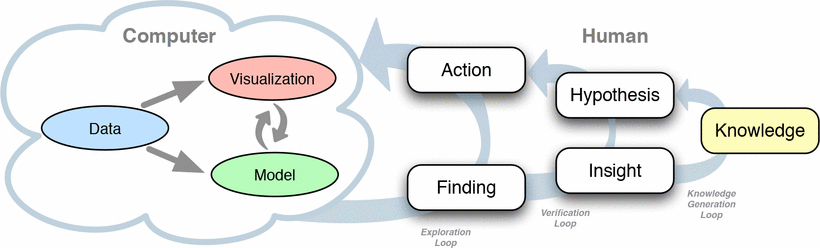
\includegraphics[width=0.75\linewidth]{poster_idr01_UNamur_2017/figures/ml_with_human.png}\\
    \tiny{Figure: Visual analytic with Human-in-the-loop \cite{Sacha2017Interaction}}
\end{tabular}
\end{center}
\qquad\textbf{Research questions}:
\begin{itemize}
    \compresslist
    \item How to {\color{blue} integrate human knowledge} into the DR methods?
    \item How the user's {\color{blue} cognitive feedback} are translated to the {\color{blue} parametric constraints} used in the DR algorithms?
\end{itemize}
\end{minipage}
}

% --------------------------------------------------------------------------- %
\headerbox{Different Approaches for Integrating User Constraints}{name=constraint, column=0,span=4,below=interactiveDR}{
Feedback from users can be seen as \textbf{constraints} at different levels:
\textbf{Instance-level}$^{[A]}$,
\textbf{Group-level}$^{[B]}$,
\textbf{Feature-level}$^{[C]}$,
and \textbf{Dataset-level}$^{[D]}$.

\begin{multicols}{3}
    \section*{Feature exploration \small{($[A],[C]$)}}
    \begin{center}
        \begin{tabular}{c}
            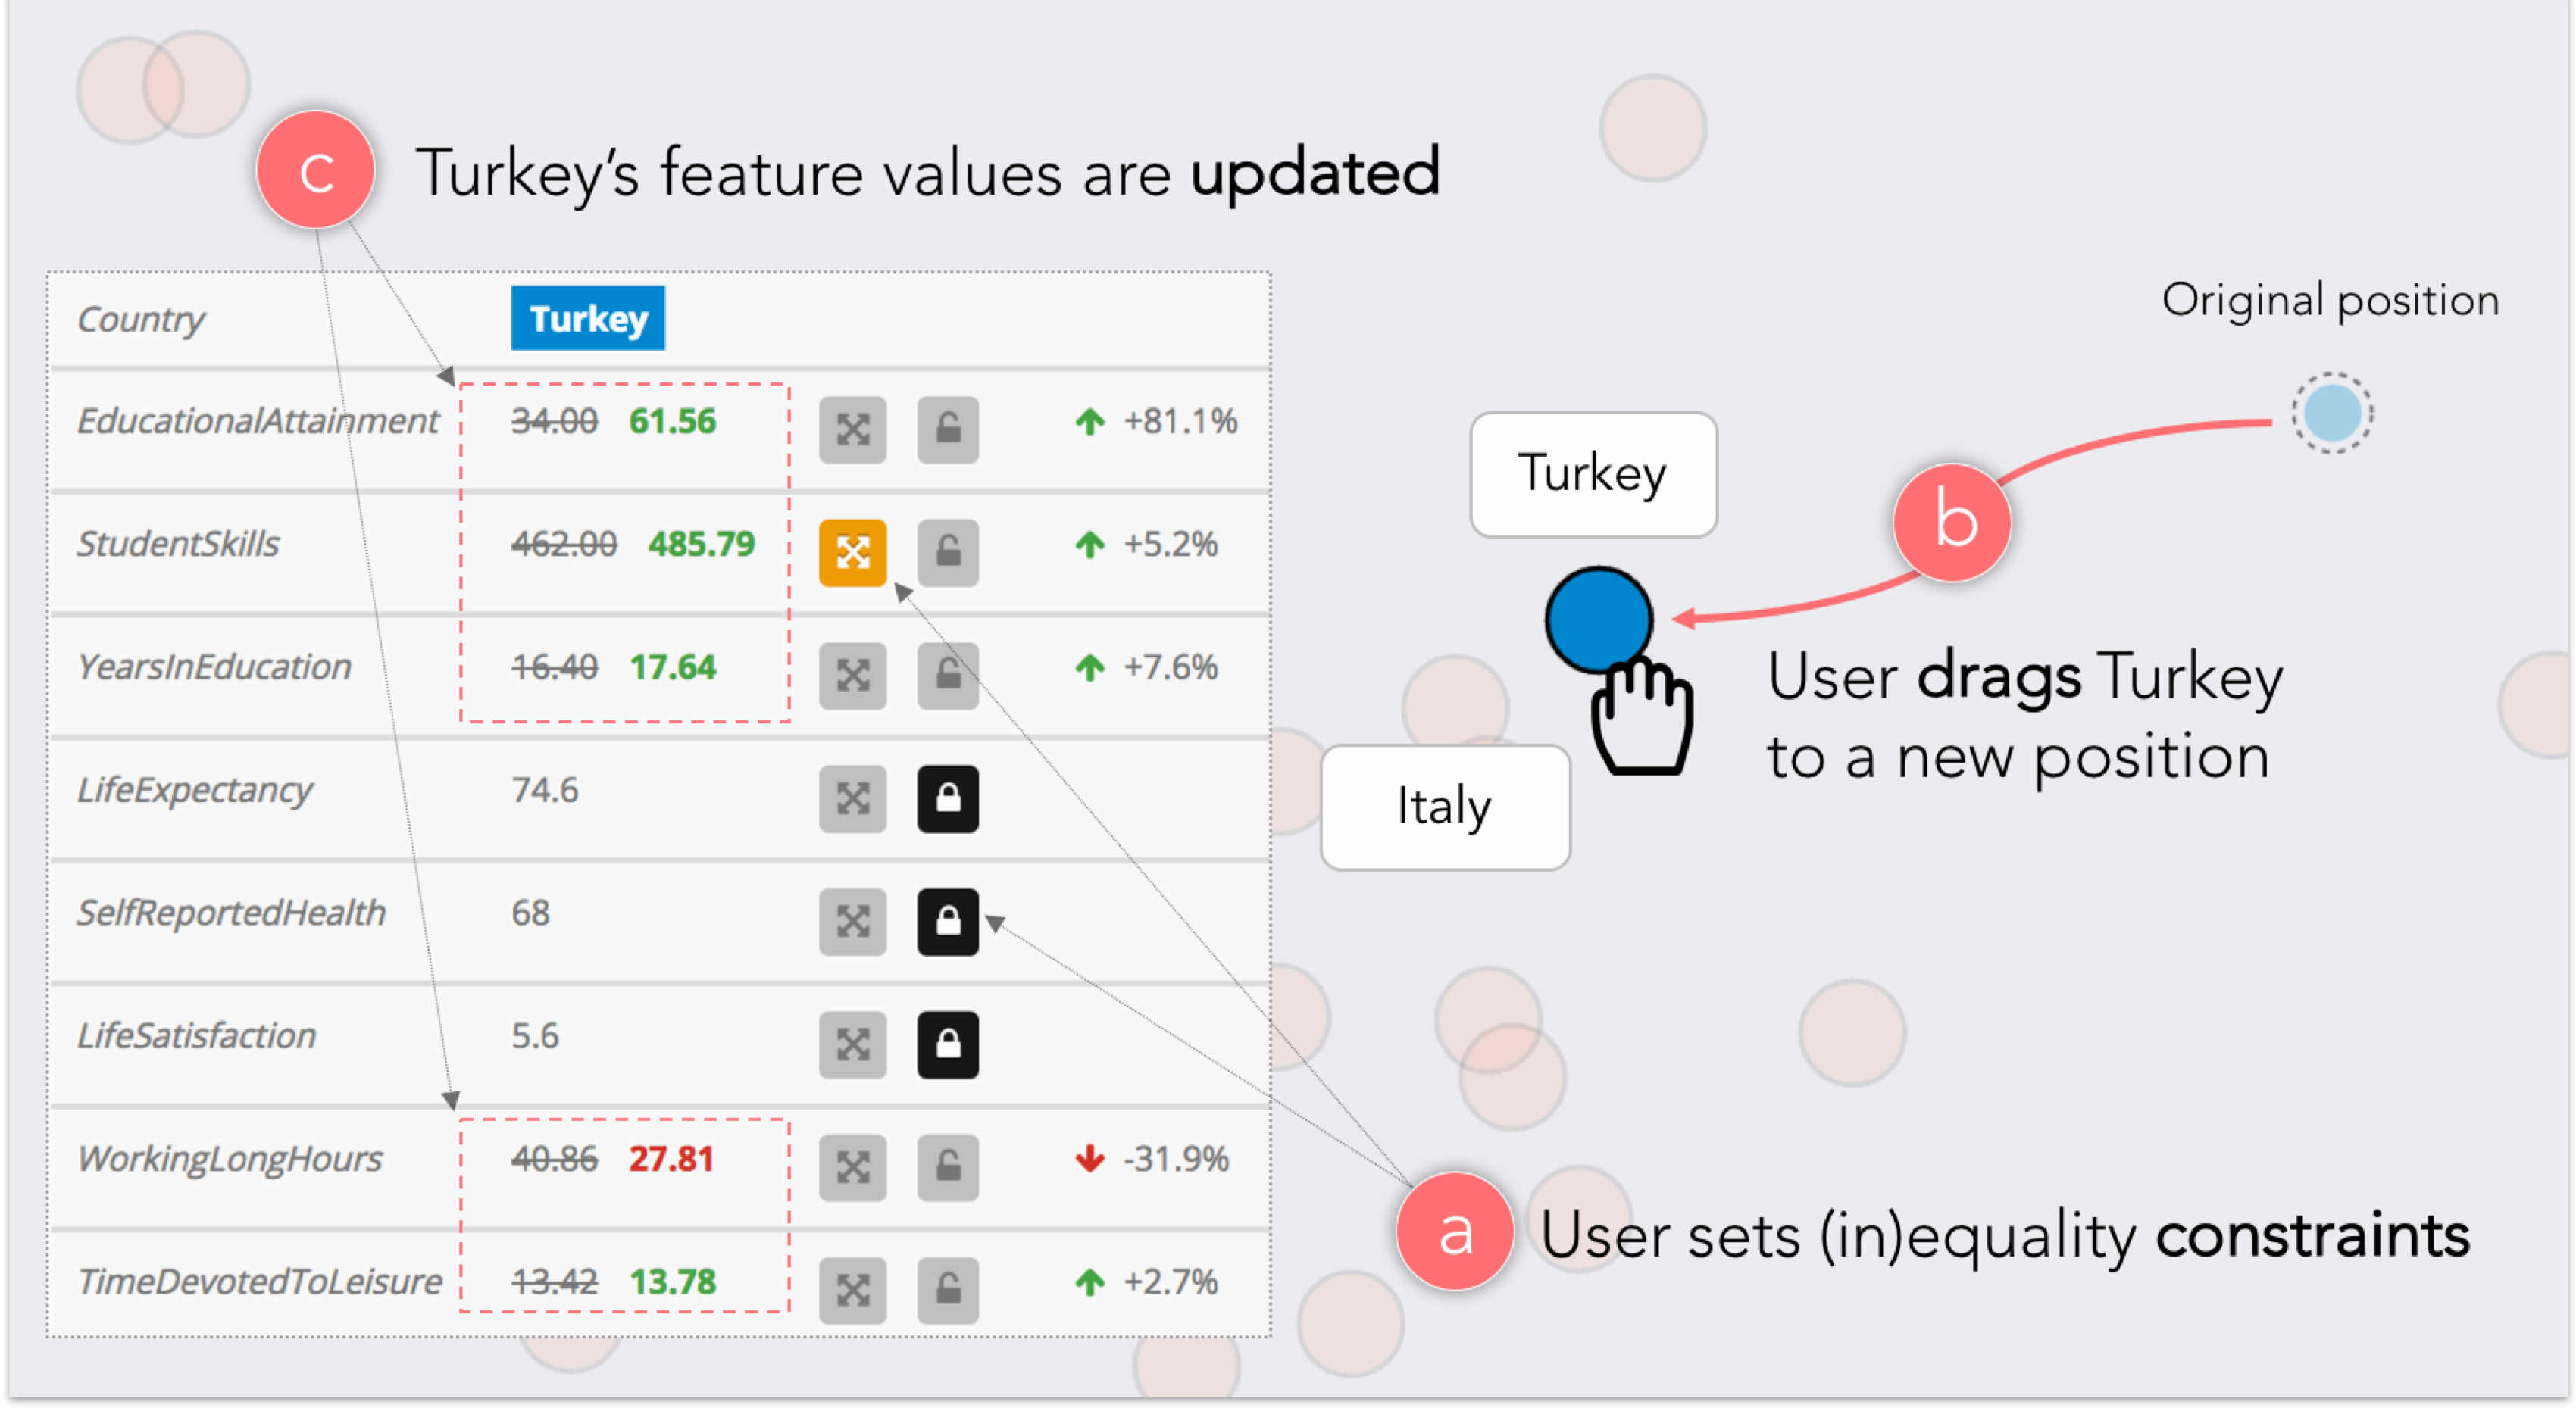
\includegraphics[height=8em]{poster_NADI_2018/images/eg_forward_backward.png}\\
            \tiny{Figure: Forward and Backward Projections \cite{cavallo2017FWBW}}
        \end{tabular}
        \begin{tabular}{p{20em}}
            \quad Move points to see how the values of their features change.
            \pointer
            Understand which features determine the position of points.% in the visualization.
        \end{tabular}
    \end{center}

    \section*{\small{Triplet constraints (\small{$[A],[B]$})}}
    \begin{center}
        \begin{tabular}{c}
            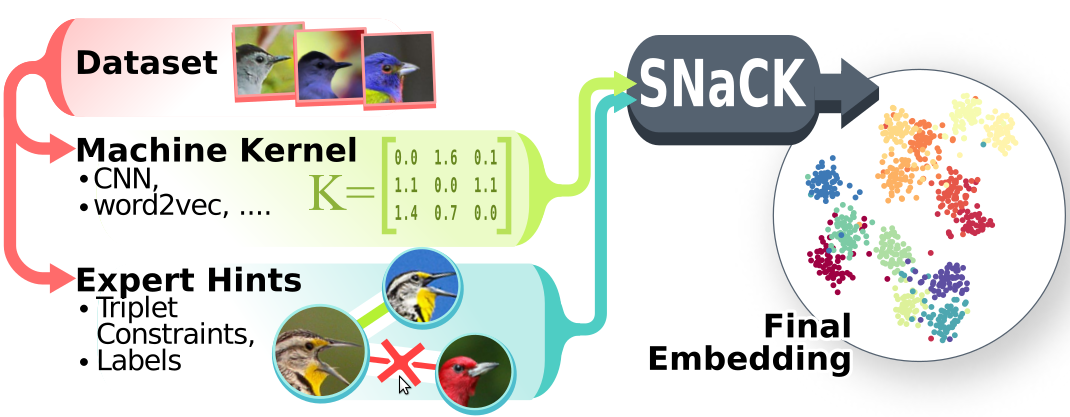
\includegraphics[height=8em]{poster_NADI_2018/images/eg_triplet.png}\\
            \tiny{Figure: Stochastic Triplet Embedding \cite{van2012ste}}
        \end{tabular}
        \begin{tabular}{p{22em}}
            \quad\texttt{Triplet} $(i, j, k)$: object $i$ seems more similar to object $j$ than to object $k$.
            \pointer
            Help experts explore and label the dataset in an interactive manner.
        \end{tabular}
    \end{center}

    \section*{\small{Example-based constraints (\small{$[B],[C],[D]$})}}
    \begin{center}
        \begin{tabular}{c}
            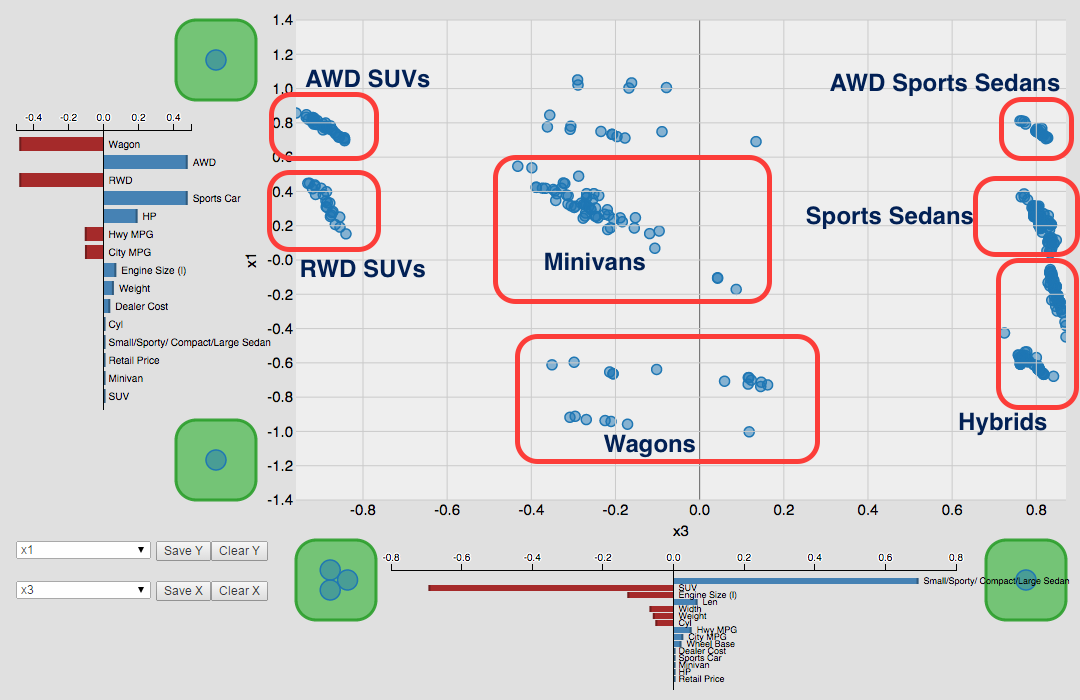
\includegraphics[height=8em]{poster_NADI_2018/images/eg_interaxis.png}\\
            \tiny{Figure: InterAxis: Steering Scatterplot Axes \cite{Kim2016InterAxis}}
        \end{tabular}
        \begin{tabular}{p{13em}}
            \quad Using examples to guide the algorithm to construct two easy understandable axes.
        \end{tabular}
    \end{center}
\end{multicols}
}

% --------------------------------------------------------------------------- %
\headerbox{Proposed Interactive t-SNE Method}{name=method, column=0,span=4,below=constraint}{
\begin{center}
\begin{tabular}{c}
    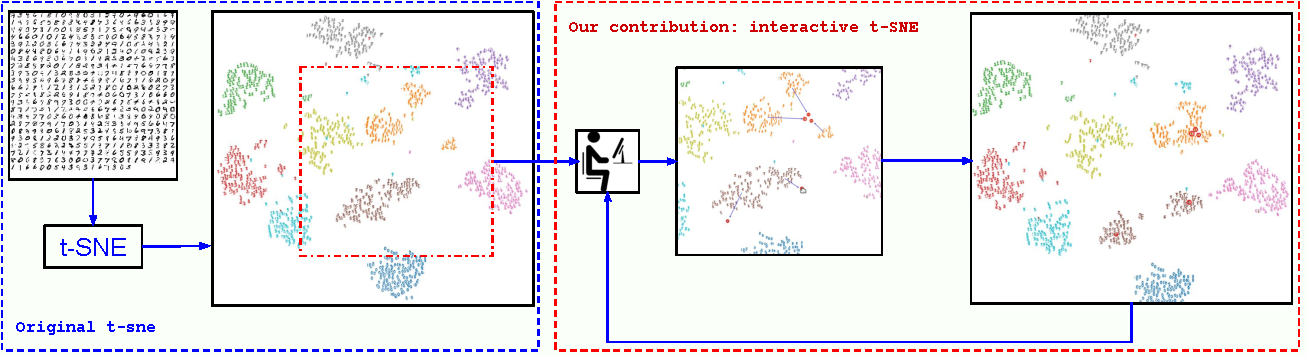
\includegraphics[width=0.95\linewidth]{poster_NADI_2018/images/tsnex.pdf}\\
    % \tiny{Figure: }
\end{tabular}
\end{center}

\begin{minipage}{0.52\linewidth}
\noindent
\begin{itemize}
    \item \textbf{Idea}: Extend $t$-SNE, a widely used DR method, to take into account the user's feedback. User moves points to control the groups:
    \noindent
    \begin{itemize}
        % \compresslist
        \item Moving points close together to merge the small, similar clusters. \small{\color{blue}{(a)}}
        \item Moving points far apart to divide up a large cluster. \small{\color{blue}{(b)}}
    \end{itemize}
\end{itemize}
\end{minipage}
\begin{minipage}{0.44\linewidth}
\noindent
\begin{itemize}
    \item \textbf{How it works}: Add a {\color{red} penalty term} to the objective function of $t$-SNE to force the \emph{neighbors} of the selected points follow these points when they are moved.
    \item \textbf{Points to improve}: Choose the important points to interact with and find an interpretable, parameter-free penalty term.
\end{itemize}
\end{minipage}
}

% --------------------------------------------------------------------------- %
\headerbox{References}{name=ref,column=0,span=4,below=method}{
\scriptsize % Reduce the font size in this block
\renewcommand{\section}[2]{\vskip 0.0em} % Get rid of the default "References" section title
% \nocite{*} % Insert publications even if they are not cited in the poster
\bibliographystyle{abbrv}
\bibliography{refs} % Use sample.bib as the bibliography file
}


\end{poster}

\end{document}

